\section{Strain Gauge and iRotor Sensor Fusion}
Although the analysis so far compares the use of either root strain gauges or tip deflection sensors, it is also valuable to investigate using both sensors in conjunction with each other. Using both sensors provides information about the root and the tip of the blade, which allows for better approximation of the state of the blade system. Whereas using one sensor allows for the first blade mode to be observed, using two sensors allows for the first two blade modes to be observed. To demonstrate this, consider the full equation for tip deflection, $y(t)$ and root bending moment, $M(t)$ derived in section XX:
\begin{align}
    M(t) &= EI_0\sum_{i=1}^\infty \alpha_i(t) \left.\frac{\partial ^2 \gamma_i}{\partial z^2}\right\vert_{z=0}\\
    y(t) &= \sum_{i=1}^\infty \alpha_i(t)
\end{align}

Now, considering only the first two modes ($i = 1, 2$), a linear set of equations connecting tip deflection, root bending moment and the first two mode amplitudes can be formed. For brevity, the following notation is introduced: $\gamma_i '' = \left.\frac{\partial ^2 \gamma_i}{\partial z^2}\right\vert_{z=0}$
\begin{equation}
    \begin{bmatrix}
    M(t) \\ y(t)
    \end{bmatrix}
    =     \begin{bmatrix}
    EI_0\gamma_1'' & EI_0\gamma_2'' \\
    1 & 1
    \end{bmatrix}
        \begin{bmatrix}
    \alpha_1(t) \\ \alpha_2(t)
    \end{bmatrix}
\end{equation}
As the mode shapes are orthogonal, the curvature terms are not equal. Therefore the matrix is invertible, and therefore a transformation between state space and modal space can be found:
\begin{equation}
        \begin{bmatrix}
    \alpha_1(t) \\ \alpha_2(t)
    \end{bmatrix}
    =    
    \begin{bmatrix}
    \frac{1}{EI_0(\gamma_1'' - \gamma_2'')} & -\frac{\gamma_2''}{\gamma_1'' - \gamma_2''} \\
    -\frac{1}{EI_0(\gamma_1'' - \gamma_2'')} & \frac{\gamma_1''}{\gamma_1'' - \gamma_2''}
    \end{bmatrix}
 \begin{bmatrix}
    M(t) \\ y(t)
    \end{bmatrix}
\end{equation}
Therefore
\begin{equation}
    u(t, z) \approx \frac{\gamma_1 - \gamma_2}{EI_0(\gamma_1'' - \gamma_2'')}M_0(t) + \frac{\gamma_1''\gamma_2 - \gamma_2''\gamma_1}{\gamma_1'' - \gamma_2''}y(t)
\end{equation}



\section{Full Blade Deflection Estimation}
By measuring the amplitude of the first two modes, the flapwise blade deformation along the entire blade can be estimated if the first two mode shapes are known. The deformation of the entire blade could be useful in estimating the wind field, the force distribution along the blade, and for better control system modelling. Although the implementation of these suggestions is not carried out in this project, a brief comparison of the different estimation methods is outlined in this section.
\begin{equation}
    \tilde{u}_{\text{TD, RBM}}(t, z) \approx \frac{\gamma_1 - \gamma_2}{EI_0(\gamma_1'' - \gamma_2'')}(M_0(t) + C_1) + \frac{\gamma_1''\gamma_2 - \gamma_2''\gamma_1}{\gamma_1'' - \gamma_2''}(y(t) - y_p)
\end{equation}
It was found that adding an constant offset, $C_1$, to the RBM measurement to account for steady error yielded better results. The tip deflection measurement is also offset by the amount of prebend in the blade, $y_0$. This estimation is compared to using a single tip deflection sensor and a single RBM sensor. The equations for these estimation are derived from XX as follows:
\begin{align}
    \tilde{u}_{\text{TD}}(t, z) &\approx \gamma_1(y(t) - y_p) \\
    \tilde{u}_{\text{RBM}}(t, z) &\approx \frac{\gamma_1}{EI_0\gamma_1''}(M(t) - C_2)
\end{align}
To test the accuracy of this estimation, a HAWC2 simulation is run on the DTU10MW turbine model at a windspeed of 12m/s under with NTM (check if this abbreviation has been defined) for 30 minutes with position sensors along the entire length of the blade. 

To evaluate the performance, the mean square error, $E$, is determined for each estimation. That is,
\begin{equation}
    E = \frac{1}{N} \sum_{i=1}^N \left( u_i(z) - \tilde{u}_i(z)\right)^2
\end{equation}
The constant offsets, $C_1$ and $C_2$ were found such that the mean square error is minimised. The Mean square error of these estimations are shown in Table XX. A tip deflection sensor is able to provide a better estimate of the blade deformation than an RBM sensor, however, using both sensors together provides a better overall result. Figures XX show the worst case estimations for each of the sensors. The RBM sensor tends to poorly estimate the deformation behaviour towards the blade tip. Discrepancies in the estimation are likely from higher mode excitation and non-linear bending. These factors could be accounted for by including additional sensors along the span of the blade and by using different blade modelling equations such as Timoshenko beam theory.

\begin{figure}[H] 

	\makebox[\textwidth][c]{
    \begin{subfigure}[b]{0.4\textwidth}
    \centering
    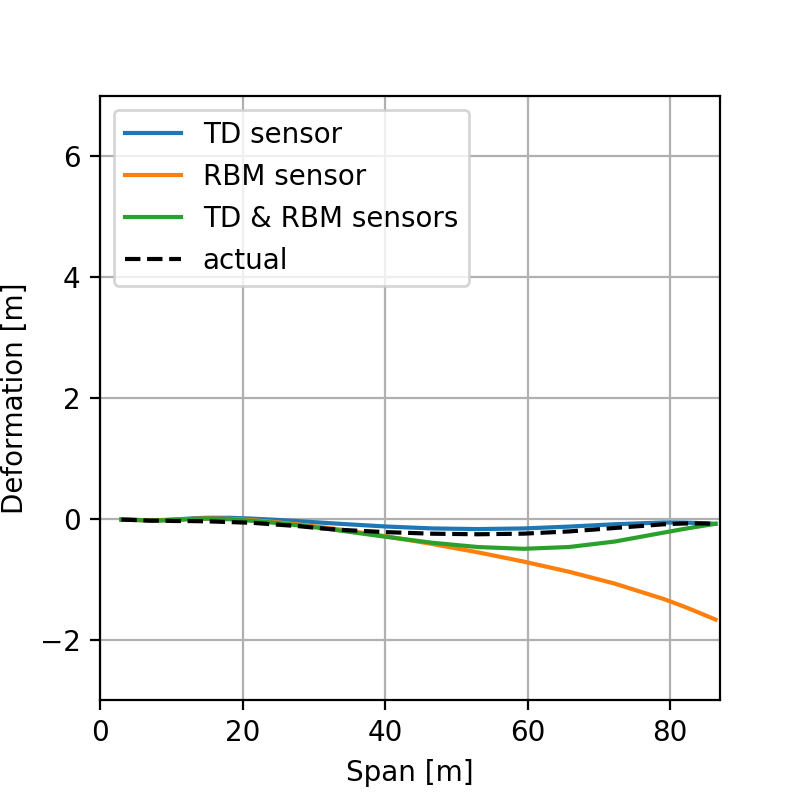
\includegraphics[width=1\textwidth]{Figures/TD_RBM_BladeDeformationEstimation.png}
    \caption{\small a}
	\label{#3}
    \end{subfigure}
    \begin{subfigure}[b]{0.4\textwidth}
    
    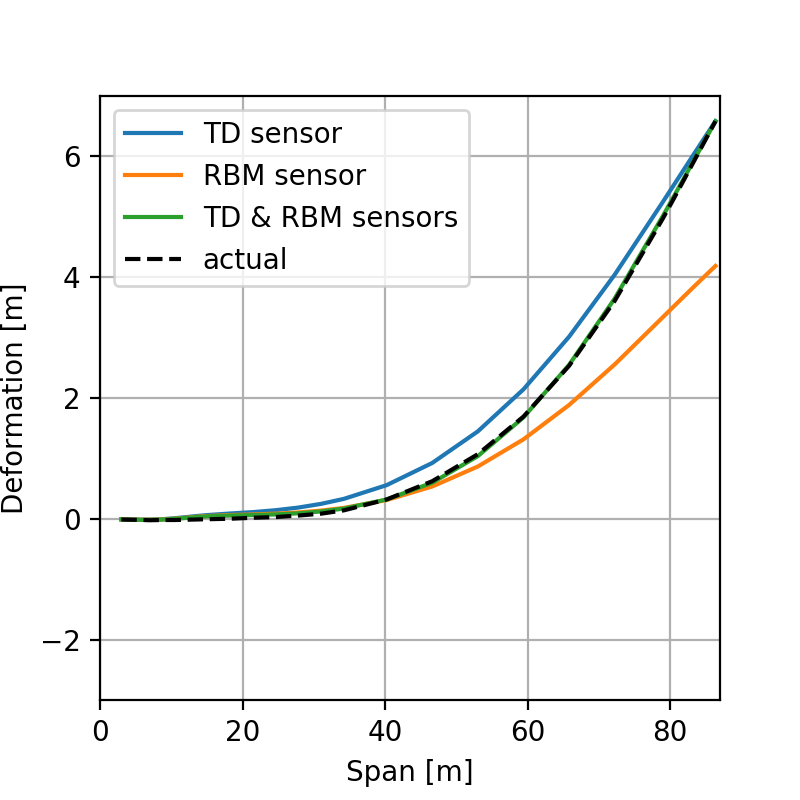
\includegraphics[width=1\textwidth]{TD_BladeDeformationEstimation.png}
    \caption{\small a}
	\label{#6}
    \end{subfigure}   
    \begin{subfigure}[b]{0.4\textwidth}
    
    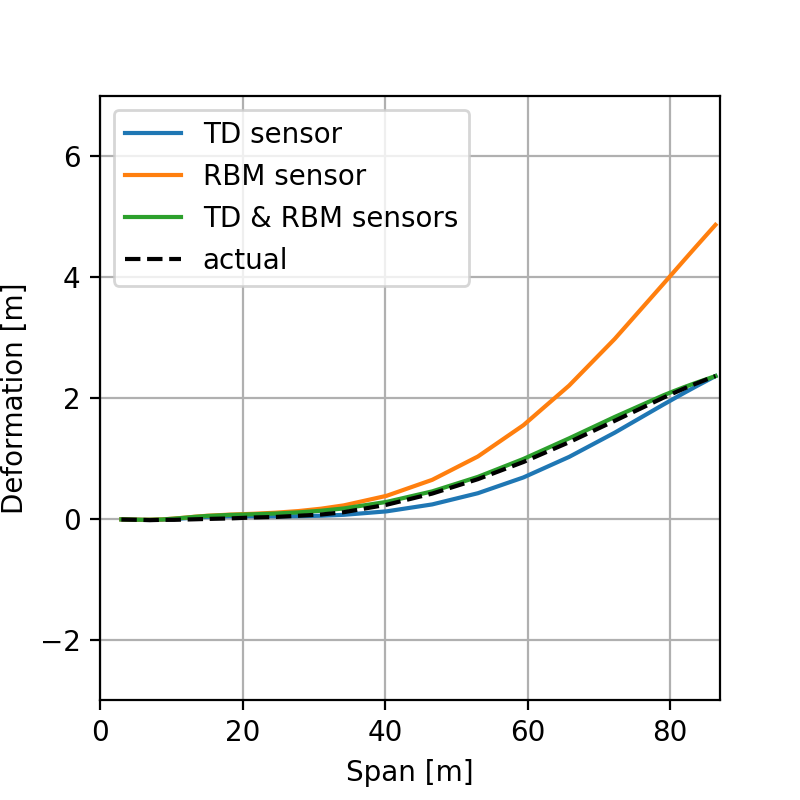
\includegraphics[width=1\textwidth]{RBM_BladeDeformationEstimation.png}
    \caption{\small a}
	\label{#6}
    \end{subfigure} 
    }
 	\setlength\fboxsep{1pt}
 	\setlength\fboxrule{0.5pt}
	\caption{\small a}
	\label{#8}
\end{figure}